\documentclass[14pt]{extbook}
\usepackage{multicol, enumerate, enumitem, hyperref, color, soul, setspace, parskip, fancyhdr} %General Packages
\usepackage{amssymb, amsthm, amsmath, bbm, latexsym, units, mathtools} %Math Packages
\everymath{\displaystyle} %All math in Display Style
% Packages with additional options
\usepackage[headsep=0.5cm,headheight=12pt, left=1 in,right= 1 in,top= 1 in,bottom= 1 in]{geometry}
\usepackage[usenames,dvipsnames]{xcolor}
\usepackage{dashrule}  % Package to use the command below to create lines between items
\newcommand{\litem}[1]{\item#1\hspace*{-1cm}\rule{\textwidth}{0.4pt}}
\pagestyle{fancy}
\lhead{Progress Quiz 4}
\chead{}
\rhead{Version A}
\lfoot{8448-1521}
\cfoot{}
\rfoot{Fall 2020}
\begin{document}

\begin{enumerate}
\litem{
Which of the following equations \textit{could} be of the graph presented below?
\begin{center}
    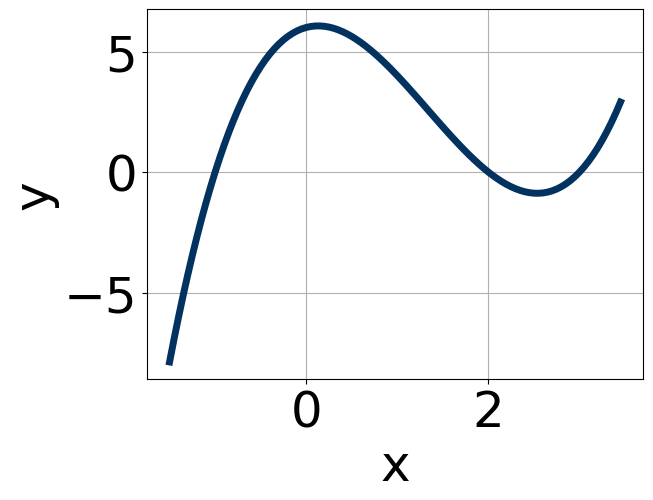
\includegraphics[width=0.5\textwidth]{../Figures/polyGraphToFunctionCopyA.png}
\end{center}
\begin{enumerate}[label=\Alph*.]
\item \( -5(x + 2)^{6} (x - 1)^{8} (x + 3)^{11} \)
\item \( 12(x + 2)^{6} (x - 1)^{10} (x + 3)^{5} \)
\item \( 7(x + 2)^{10} (x - 1)^{10} (x + 3)^{8} \)
\item \( -7(x + 2)^{6} (x - 1)^{7} (x + 3)^{7} \)
\item \( -5(x + 2)^{6} (x - 1)^{4} (x + 3)^{10} \)

\end{enumerate} }
\litem{
Construct the lowest-degree polynomial given the zeros below. Then, choose the intervals that contain the coefficients of the polynomial in the form $x^3+bx^2+cx+d$.\[ 2 + 5 i \text{ and } -4 \]\begin{enumerate}[label=\Alph*.]
\item \( b \in [0.16, 1.34], c \in [0, 5], \text{ and } d \in [-9, -3] \)
\item \( b \in [-1.51, 0.14], c \in [4, 21], \text{ and } d \in [-119, -107] \)
\item \( b \in [-1.51, 0.14], c \in [4, 21], \text{ and } d \in [112, 121] \)
\item \( b \in [0.16, 1.34], c \in [-2, 0], \text{ and } d \in [-20, -14] \)
\item \( \text{None of the above.} \)

\end{enumerate} }
\litem{
Which of the following equations \textit{could} be of the graph presented below?
\begin{center}
    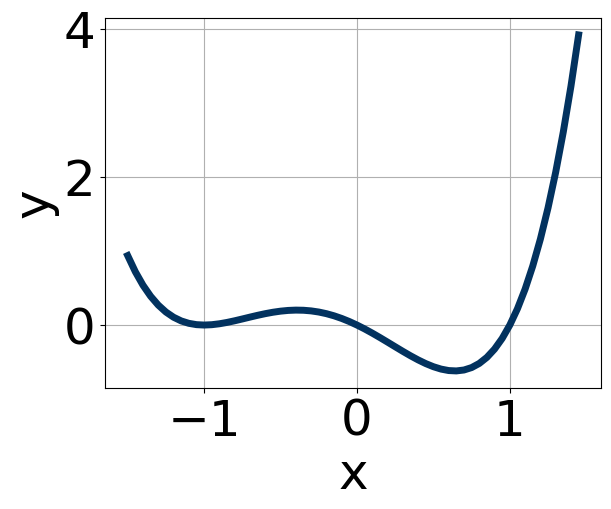
\includegraphics[width=0.5\textwidth]{../Figures/polyGraphToFunctionA.png}
\end{center}
\begin{enumerate}[label=\Alph*.]
\item \( -16x^{10} (x + 2)^{5} (x - 1)^{5} \)
\item \( -14x^{10} (x + 2)^{8} (x - 1)^{7} \)
\item \( -15x^{5} (x + 2)^{4} (x - 1)^{9} \)
\item \( 8x^{4} (x + 2)^{11} (x - 1)^{8} \)
\item \( 2x^{4} (x + 2)^{5} (x - 1)^{11} \)

\end{enumerate} }
\litem{
Describe the zero behavior of the zero $x = -3$ of the polynomial below.\[ f(x) = -3(x + 3)^{2}(x - 3)^{5}(x + 4)^{9}(x - 4)^{10} \]\begin{enumerate}[label=\Alph*.]
\begin{multicols}{2}\item 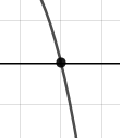
\includegraphics[width = 0.3\textwidth]{../Figures/polyZeroBehaviorAA.png}\item 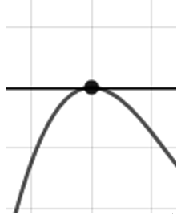
\includegraphics[width = 0.3\textwidth]{../Figures/polyZeroBehaviorBA.png}\item 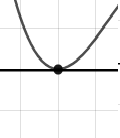
\includegraphics[width = 0.3\textwidth]{../Figures/polyZeroBehaviorCA.png}\item 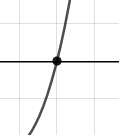
\includegraphics[width = 0.3\textwidth]{../Figures/polyZeroBehaviorDA.png}\end{multicols}\item None of the above.
\end{enumerate} }
\litem{
Describe the zero behavior of the zero $x = 5$ of the polynomial below.\[ f(x) = 9(x + 5)^{5}(x - 5)^{10}(x + 7)^{9}(x - 7)^{12} \]\begin{enumerate}[label=\Alph*.]
\begin{multicols}{2}\item 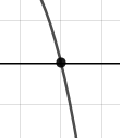
\includegraphics[width = 0.3\textwidth]{../Figures/polyZeroBehaviorCopyAA.png}\item 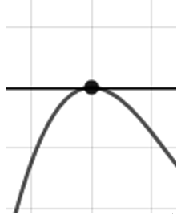
\includegraphics[width = 0.3\textwidth]{../Figures/polyZeroBehaviorCopyBA.png}\item 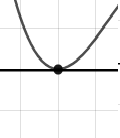
\includegraphics[width = 0.3\textwidth]{../Figures/polyZeroBehaviorCopyCA.png}\item 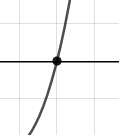
\includegraphics[width = 0.3\textwidth]{../Figures/polyZeroBehaviorCopyDA.png}\end{multicols}\item None of the above.
\end{enumerate} }
\litem{
Describe the end behavior of the polynomial below.\[ f(x) = 9(x - 4)^{4}(x + 4)^{9}(x - 6)^{4}(x + 6)^{4} \]\begin{enumerate}[label=\Alph*.]
\begin{multicols}{2}\item 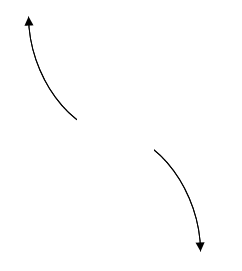
\includegraphics[width = 0.3\textwidth]{../Figures/polyEndBehaviorCopyAA.png}\item 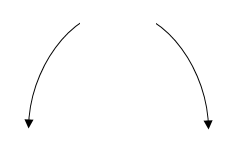
\includegraphics[width = 0.3\textwidth]{../Figures/polyEndBehaviorCopyBA.png}\item 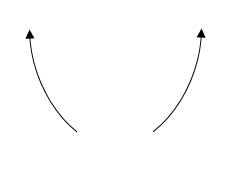
\includegraphics[width = 0.3\textwidth]{../Figures/polyEndBehaviorCopyCA.png}\item 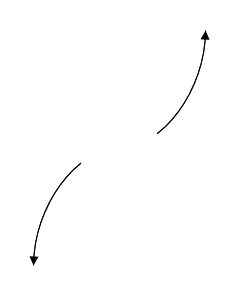
\includegraphics[width = 0.3\textwidth]{../Figures/polyEndBehaviorCopyDA.png}\end{multicols}\item None of the above.
\end{enumerate} }
\litem{
Describe the end behavior of the polynomial below.\[ f(x) = -9(x - 9)^{2}(x + 9)^{3}(x - 4)^{2}(x + 4)^{4} \]\begin{enumerate}[label=\Alph*.]
\begin{multicols}{2}\item 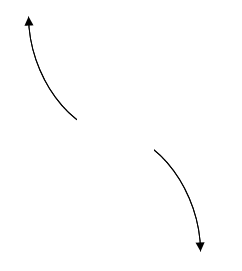
\includegraphics[width = 0.3\textwidth]{../Figures/polyEndBehaviorAA.png}\item 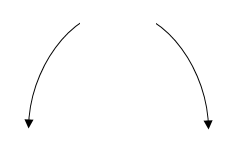
\includegraphics[width = 0.3\textwidth]{../Figures/polyEndBehaviorBA.png}\item 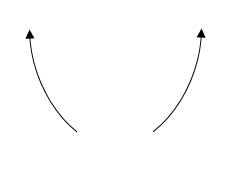
\includegraphics[width = 0.3\textwidth]{../Figures/polyEndBehaviorCA.png}\item 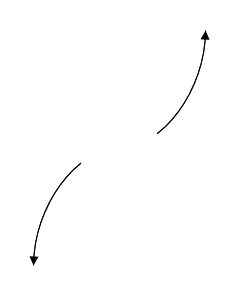
\includegraphics[width = 0.3\textwidth]{../Figures/polyEndBehaviorDA.png}\end{multicols}\item None of the above.
\end{enumerate} }
\litem{
Construct the lowest-degree polynomial given the zeros below. Then, choose the intervals that contain the coefficients of the polynomial in the form $ax^3+bx^2+cx+d$.\[ \frac{-2}{5}, \frac{3}{5}, \text{ and } \frac{2}{3} \]\begin{enumerate}[label=\Alph*.]
\item \( a \in [74, 76], b \in [58, 66], c \in [-12, -2], \text{ and } d \in [-18, -4] \)
\item \( a \in [74, 76], b \in [-36, -34], c \in [-30, -26], \text{ and } d \in [12, 17] \)
\item \( a \in [74, 76], b \in [-70, -60], c \in [-12, -2], \text{ and } d \in [12, 17] \)
\item \( a \in [74, 76], b \in [-129, -119], c \in [61, 70], \text{ and } d \in [-18, -4] \)
\item \( a \in [74, 76], b \in [-70, -60], c \in [-12, -2], \text{ and } d \in [-18, -4] \)

\end{enumerate} }
\litem{
Construct the lowest-degree polynomial given the zeros below. Then, choose the intervals that contain the coefficients of the polynomial in the form $ax^3+bx^2+cx+d$.\[ \frac{-7}{5}, \frac{3}{4}, \text{ and } \frac{-3}{2} \]\begin{enumerate}[label=\Alph*.]
\item \( a \in [40, 44], b \in [-92, -83], c \in [-5, 1], \text{ and } d \in [59, 64] \)
\item \( a \in [40, 44], b \in [85, 87], c \in [-5, 1], \text{ and } d \in [-67, -58] \)
\item \( a \in [40, 44], b \in [30, 40], c \in [-84, -78], \text{ and } d \in [-67, -58] \)
\item \( a \in [40, 44], b \in [-27, -22], c \in [-87, -82], \text{ and } d \in [59, 64] \)
\item \( a \in [40, 44], b \in [85, 87], c \in [-5, 1], \text{ and } d \in [59, 64] \)

\end{enumerate} }
\litem{
Construct the lowest-degree polynomial given the zeros below. Then, choose the intervals that contain the coefficients of the polynomial in the form $x^3+bx^2+cx+d$.\[ 3 - 5 i \text{ and } 3 \]\begin{enumerate}[label=\Alph*.]
\item \( b \in [-14, -5], c \in [51, 58], \text{ and } d \in [-109, -97] \)
\item \( b \in [4, 16], c \in [51, 58], \text{ and } d \in [99, 103] \)
\item \( b \in [-1, 4], c \in [1, 3], \text{ and } d \in [-17, -10] \)
\item \( b \in [-1, 4], c \in [-19, -3], \text{ and } d \in [5, 11] \)
\item \( \text{None of the above.} \)

\end{enumerate} }
\end{enumerate}

\end{document}